%
\documentclass[a4paper]{article}


\usepackage{color}              %Farben, f.r \definecolor{}
\usepackage{amssymb}            %Mathematische Symbole
\usepackage{amsthm}             %Besseres \newtheorem
\usepackage{amsmath}           %Mathematische Umgebungen
\usepackage{mathtools}          %\xRightarrow, etc
\usepackage{mathrsfs}           %enthaelt \mathscr
\usepackage[matrix,arrow,curve]{xy}     %Diagramme
\usepackage{graphicx}
\usepackage{enumerate}          % in-place numerations def.
\usepackage{fullpage}

\newcommand{\RR}{\mathbb{R}}
\newcommand{\ZZ}{\mathbb{Z}}

%% Dokument Beginn %%%%%%%%%%%%%%%%%%%%%%%%%%%%%%%%%%%%%%%%%%%%%%%%%%%%%%%%
\begin{document}
\pagestyle{empty}
\begin{center}
	{\Large\bf Graph coloring}\\
	{\large\bf Exercise class problems - volume 6}\\
	\line(1,0){330}
\end{center}

Edge-chromatic numbers, from last week:

\begin{enumerate}
\item If $G$ is connected and $L(G)$ is isomorphic to $G$ then $G$ is a cycle.
\item Suppose $G$ is $r$-regular with an odd number of vertices. Prove that $r$ is even and that $\chi'(G)=r+1$.
\item Find the edge-chromatic number of the Petersen graph.
\end{enumerate}

Coloring Euclidean spaces:

\begin{enumerate}
%\item Turn our proof of $\chi(\RR^2)\geq 4$ into a construction of an explicit finite graph $H\subseteq U_{\RR^2}$ with $\chi(H)=4$.
\item What is $\omega(U_{\RR^2})$\ ?

\item What is the length of the side in a $d$-dimensional cube whose main diagonal has length $1$?

\item Recall our naive coloring of $U_{\RR^2}$ by translates of a $9$-colored $3\times 3$ square, where each small square has diameter almost $1$:

\begin{center}
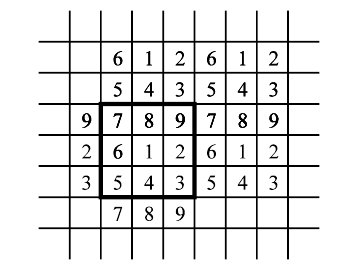
\includegraphics[scale=0.4]{mf8.png}
\end{center}

Does the same strategy work in $\RR^3$ and produce a coloring of $U_{\RR^3}$ with $27$ colors by translates of a $27$-colored $3\times 3\times 3$ cube? What about $\RR^d$\ 	?

\item These figures have all got something to do with the bounds $4\leq\chi(\RR^2)\leq 7$. Explain (or wait until the lecture tomorrow).

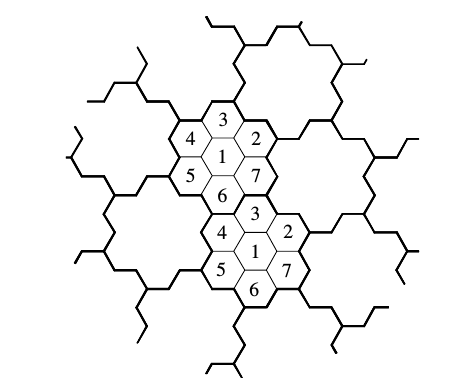
\includegraphics[scale=0.5]{mf5.png}  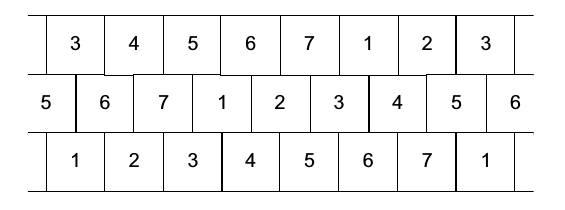
\includegraphics[scale=0.5]{mf9.png}

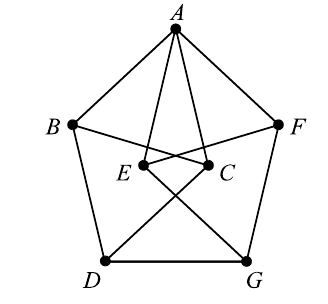
\includegraphics[scale=0.4]{mf6.png} 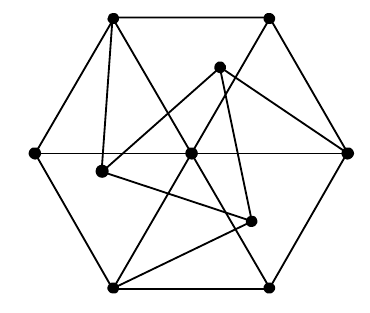
\includegraphics[scale=0.4]{mf7.png}


\end{enumerate}

Bonus:

\begin{enumerate}
\item We say that two points $A$ and $B$ of the integer lattice $\ZZ^2$ \emph{see each other} if the line segment $AB$ contains no other point of $\ZZ^2$. Find a $4$-coloring of $\ZZ^2$ so that any two points which see each other have different colors. Hint: use colors $00, 01, 10, 11$.
\end{enumerate}

\end{document}




